%% Version 4.3.2, 25 August 2014
%
%%%%%%%%%%%%%%%%%%%%%%%%%%%%%%%%%%%%%%%%%%%%%%%%%%%%%%%%%%%%%%%%%%%%%%
% Template.tex --  LaTeX-based template for submissions to the 
% American Meteorological Society
%
% Template developed by Amy Hendrickson, 2013, TeXnology Inc., 
% amyh@texnology.com, http://www.texnology.com
% following earlier work by Brian Papa, American Meteorological Society
%
% Email questions to latex@ametsoc.org.
%
%%%%%%%%%%%%%%%%%%%%%%%%%%%%%%%%%%%%%%%%%%%%%%%%%%%%%%%%%%%%%%%%%%%%%
%  PREAMBLE
%%%%%%%%%%%%%%%%%%%%%%%%%%%%%%%%%%%%%%%%%%%%%%%%%%%%%%%%%%%%%%%%%%%%%

%% Start with one of the following:
%  DOUBLE-SPACED VERSION FOR SUBMISSION TO THE AMS
\documentclass{ametsoc}

%  TWO-COLUMN JOURNAL PAGE LAYOUT---FOR AUTHOR USE ONLY
%\documentclass[twocol]{ametsoc}

\usepackage{multirow}
\usepackage{gensymb}
% \usepackage[disable]{todonotes} % notes not showed
\usepackage[prependcaption,textsize=small]{todonotes}   % notes showed

%%%%%%%%%%%%%%%%%%%%%%%%%%%%%%%%
%%% To be entered only if twocol option is used

\journal{jcli}

%  Please choose a journal abbreviation to use above from the following list:
% 
%   jamc     (Journal of Applied Meteorology and Climatology)
%   jtech     (Journal of Atmospheric and Oceanic Technology)
%   jhm      (Journal of Hydrometeorology)
%   jpo     (Journal of Physical Oceanography)
%   jas      (Journal of Atmospheric Sciences)	
%   jcli      (Journal of Climate)
%   mwr      (Monthly Weather Review)
%   wcas      (Weather, Climate, and Society)
%   waf       (Weather and Forecasting)
%   bams (Bulletin of the American Meteorological Society)
%   ei    (Earth Interactions)

%%%%%%%%%%%%%%%%%%%%%%%%%%%%%%%%
%Citations should be of the form ``author year''  not ``author, year''
\bibpunct{(}{)}{;}{a}{}{,}

%%%%%%%%%%%%%%%%%%%%%%%%%%%%%%%%

%%% To be entered by author:

%% May use \\ to break lines in title:

\title{Comparison of global reanalysis datasets in the context of statistical precipitation downscaling.}

%%% Enter authors' names, as you see in this example:
%%% Use \correspondingauthor{} and \thanks{Current Affiliation:...}
%%% immediately following the appropriate author.
%%%
%%% Note that the \correspondingauthor{} command is NECESSARY.
%%% The \thanks{} commands are OPTIONAL.

    %\authors{Author One\correspondingauthor{Author One, 
    % American Meteorological Society, 
    % 45 Beacon St., Boston, MA 02108.}
% and Author Two\thanks{Current affiliation: American Meteorological Society, 
    % 45 Beacon St., Boston, MA 02108.}}

\authors{Pascal Horton\correspondingauthor{University of Bern, Institute of Geography, Hallerstrasse 12, 3012 Bern, Switzerland.}, Rolf Weingartner, Stefan Br\"{o}nnimann}

%% Follow this form:
    % \affiliation{American Meteorological Society, 
    % Boston, Massachusetts.}

\affiliation{Oeschger Centre for Climate Change Research, Institute of Geography, University of Bern, Bern, Switzerland}

%% Follow this form:
    %\email{latex@ametsoc.org}

\email{pascal.horton@giub.unibe.ch}

%% If appropriate, add additional authors, different affiliations:
    %\extraauthor{Extra Author}
    %\extraaffil{Affiliation, City, State/Province, Country}

\extraauthor{Charles Obled}
\extraaffil{Institut des G\'{e}osciences de l'Environnement, Universit\'{e} de Grenoble-Alpes, Grenoble, France}


%%%%%%%%%%%%%%%%%%%%%%%%%%%%%%%%%%%%%%%%%%%%%%%%%%%%%%%%%%%%%%%%%%%%%
%  ABSTRACT
%
% Enter your abstract here
% Abstracts should not exceed 250 words in length!
%
% For BAMS authors only: If your article requires a Capsule Summary, please place the capsule text at the end of your abstract
% and identify it as the capsule. Example: This is the end of the abstract. (Capsule Summary) This is the capsule summary. 

\abstract{
	%The analogue method is a statistical downscaling method for precipitation prediction. It uses similarity in terms of synoptic-scale predictors with situations in the past in order to provide a probabilistic prediction for the day of interest. It has been used for decades in a context of weather or flood forecasting, and is more recently also applied to climate studies, whether for reconstruction of past weather conditions or future climate impact studies. In order to evaluate the relationship between synoptic scale predictors and the local weather variable of interest, e.g. precipitation, reanalysis datasets are necessary. Nowadays, the number of available reanalysis datasets increase. These are generated by different atmospheric models with different assimilation techniques and offer various spatial and temporal resolutions. A major difference between these datasets is also the length of the archive they provide. While some datasets start at the beginning of the satellite era and assimilate these data, others aim at homogeneity on a longer period and only assimilate conventional observations.
%The context of the application of analogue methods might drive the choice of an appropriate dataset, for example when the archive length is a leading criterion. However, in many studies, a reanalysis dataset is subjectively chosen, according to the user’s preferences or the ease of access. The impact of this choice on the results of the downscaling procedure is rarely considered and no comprehensive comparison has been undertaken so far.
%In order to fill this gap and to advise on the choice of appropriate datasets, nine different global reanalysis datasets were compared in seven distinct versions of analogue methods, over 300 precipitation stations in Switzerland. Significant differences in terms of prediction performance were identified. Although the impact of the reanalysis dataset on the skill score varies according to the chosen predictor, be it atmospheric circulation or thermodynamic variables, some hierarchy between the datasets is often preserved.
}


\begin{document}

%% Necessary!
\maketitle


\todo{Write abstract}
\todo{Check tenses}


%%%%%%%%%%%%%%%%%%%%%%%%%%%%%%%%%%%%%%%%%%%%%%%%%%%%%%%%%%%%%%%%%%%%%
%  MAIN BODY OF PAPER
%%%%%%%%%%%%%%%%%%%%%%%%%%%%%%%%%%%%%%%%%%%%%%%%%%%%%%%%%%%%%%%%%%%%%
%

%% In all cases, if there is only one entry of this type within
%% the higher level heading, use the star form: 
%%
% \section{Section title}
% \subsection*{subsection}
% text...
% \section{Section title}

%vs

% \section{Section title}
% \subsection{subsection one}
% text...
% \subsection{subsection two}
% \section{Section title}

%%%
% \section{First primary heading}

% \subsection{First secondary heading}

% \subsubsection{First tertiary heading}

% \paragraph{First quaternary heading}


%TODO: publish results as datasets?
%TODO: AM not sensitive to biases

\section{Introduction}

Statistical downscaling is widely used to bridge the resolution gap between climate model outputs and impact models, and to bias-correct them. Several of these methods consist in establishing an empirical statistical relationship between large-scale atmospheric variables and the local variable of interest. Following the classification of \citet{Rummukainen1997} also used in \citet{Maraun2010}, there are basically two types of approaches: perfect prognosis, for which the relationship is calibrated on large-scale and local-scale observations, and model output statistics, for which the relationship is calibrated on model outputs for the large-scale variables and local-scale observations. In the context of perfect prognosis approaches, large-scale observations are thus needed. Global meteorological reanalyses are very useful to fulfil this role, as they provide gridded large-scale variables available at any location of the world.

Reanalyses are produced with a single version of a data assimilation system with a forecast model constrained to follow at best the observations over a long period. They provide multivariate outputs that are physically consistent, and that contain information in locations where few or no observations are available, also for variables that are not directly observed \citep{Gelaro2017}. Their accuracy depends on both the quality of the model physics and that of the analysis process, and thus indirectly of the quantity and quality of the assimilated observations \citep{Dee2011a}. The homogeneity of a reanalysis is a challenge due to significant changes in observing systems. For example, the availability of satellite observations drastically changed the amount of data available, particularly for regions with sparse conventional observation networks. The assimilation of a variable amount of observations is likely to lead to inhomogeneities in the reanalysis. For this reason, some reanalyses are either limited to the satellite era, or, if the period of interest expands before 1980, they might not use satellite observations. Because of these discontinuities in the available observations, some variables, such as precipitation and evaporation are to be used with great caution \citep{Kobayashi2015}.

In perfect prognosis methods, reanalyses are considered as observations of the large-scale variables, and are supposed perfect. As the statistical relationship established using reanalyses is afterwards applied to outputs from other models, the variables considered as predictors should not strongly depend on the forecast model used and should be as robust as possible, so that they are mainly influenced by the observations only.

The present work focuses on the analogue method (AM), which is a statistical downscaling technique relying on the hypothesis that similar synoptic situations are likely to result in similar local effects, plus a certain variability that is not explained by the considered predictors \citep{Lorenz1969}. The variable of interest is here precipitation. In order to take into account the unexplained variability, several analogue days are selected and their observed precipitation values are used to provide the empirical conditional distribution that is the statistical prediction for the considered target day. Different versions of AMs exist, relying on various predictors. However, they generally contain a predictor describing the atmospheric circulation.

In one of the first version of the AM, the predictors were extracted from radio-sounding data \citep{Duband1981}, which involved heavy pre-treatment to have a complete and homogeneous database that could be used. Other authors worked with rather short local analysis from forecast models \cite[for example][]{Kruizinga1983, VandenDool1989}. The release of the first reanalysis dataset \citep[NCEP/NCAR Reanalysis I, NR-1,][]{Kalnay1996, Kistler2001} greatly simplified the implementation of the AM, and opened new opportunities of using other variables that were not available before. This increased the popularity of the method \citep{Timbal2008a}.

\citet{Timbal2003} and \citet{Bontron2004} were the first authors to use NR-1 in the AM. As NR-1 remained a popular dataset for a long time, this dataset or its updated version NCEP/DOE Reanalysis 2 \citep[NR-2,][]{Kanamitsu2002} were often used until recently \citep{Wetterhall2005a, Gangopadhyay2005, Altava-Ortiz2006, Barrera2007, Cannon2007, Matulla2007, Bliefernicht2007, Maurer2008, Wu2012, Marty2012, Teng2012, Horton2012, Yiou2014}. When the first European long reanalysis ERA-40 \citep{Uppala2005} became available, it also became popular for European users, but after a delay of some years \citep {Willems2011b, JakobThemessl2011a, BenDaoud2011, Turco2011a, Franke2011, Pascual2012b, Schenk2012, Ribalaygua2013a, Osca2013, Radanovics2013, Martin2014b, Chardon2014, BenDaoud2016}. \citet{BenDaoud2009} analysed the impact of choosing NR-1 or ERA-40 in the AM developed by \citet{Bontron2004} and found no significant difference for the predictors considered. The more recent ERA-Interim \citep[ERA-INT, ][]{Dee2011a} was used by \cite{Raynaud2016b}, and MERRA \citep{Rienecker2011} was used by \citet{Vanvyve2015}.

In almost all of these works, a single reanalysis was used. The choice is likely to be primarily driven by the ease of access and the availability of some datasets in the research units, along with the code able to read it. Indeed, it is often not a priority to use the last reanalysis available if the benefit for AMs is not proven, as it requires efforts to acquire ever larger datasets and to adapt the code to read it. Moreover, they are often considered as equivalent for a data-rich region such as Europe. It likely explains why many authors stick with the first American or European dataset.

Some other use of the AM focus on the reconstruction of weather conditions in the Twentieth Century. Then, they require reanalyses spanning this period, such as the Twentieth Century Reanalysis \citep[20CR][]{Compo2011} produced by NOAA \citep[for example,][]{Kuentz2015, Caillouet2016, Brigode2016}. 

To our knowledge, \citet{Dayon2015} made the most comprehensive comparison of the reanalyses in the AM so far. They compared NR-1, MERRA, ERA-INT and 20CR and noted that the choice of the reanalysis, even if not crucial for climate change impacts, is a non-negligible source of uncertainty, and that it can even impact the performance of the method to a greater extent than the choice of the predictors. They concluded that "the substantial differences in downscaling results associated with reanalyses [...] suggests that the role of reanalyses should not be underestimated when evaluating the statistical downscaling method". The choice of the predictors was also found to vary from a dataset to another, in a way that the optimization of the method is likely to be reanalysis dependent and that using a single reanalysis might introduce a lack of robustness \citep{Dayon2015}.

Reanalysis datasets were compared in multiple studies (... \todo{Add some references}), but mainly in terms of climatological properties. It is certainly important for AMs to use reanalyses with accurate climatological characteristics, and particularly a good homogeneity over the period covered. However, AMs are sensitive to daily variability, and situations related to heavy precipitation events have a large influence on the performance assessment. The impact of the reanalysis on the performance of the AM can not be directly deduced from climatological analyses and needs to be assessed within the method, which is the goal of the present work. Ten reanalyses were compared for seven AMs at 300 stations in Switzerland (Sect. \ref{sec:influence}). Additionally, the role of the dataset resolution (Sect. \ref{sec:analyzes}.\ref{sec:resolution}), the length of the archive (Sect. \ref{sec:analyzes}.\ref{sec:length}), and the use of different members from ensemble datasets (Sect. \ref{sec:analyzes}.\ref{sec:ensemble}) were investigated.


\section{Data and methods}
\label{sec:data}

\subsection{Reanalysis datasets}

The considered global atmospheric reanalysis datasets are briefly described hereafter, order chronologically, and some of their characteristics are provided in Table \ref{table:datasets}. The common period to all datasets is 1981--2010. All reanalysis products are available at a 6-h time step, with some datasets or variables having higher temporal resolution. Only the 6-h time step is considered in the present work. All reanalyses are based on observations selected after quality control, which will not be detailed here. 


\subsubsection{NCEP Reanalysis I}

The NCEP/NCAR Reanalysis I \citep[NR-1,][]{Kalnay1996, Kistler2001} was the first global reanalysis product. It was made with a forecast model frozen at the state-of-the-art of 1995 and by assimilating land surface, ship, aircraft, rawinsonde, and satellite data among others. However, upper-air observations have a much larger influence on the analysis than the surface observations \citep{Kistler2001}. The data assimilation system is a 3D variational technique (3D-Var). The model resolution is T62 (about 210~km) with 28 sigma vertical levels. All major physical processes are parameterized. The period coverage was starting first in 1957, before being extended back to 1948. \citet{Kalnay1996} were aware that assimilating all available data at a give time would have an impact on the climate of the reanalysis due to changes in the observating system, but the choice was made for accuracy over stability of the climate. A comparison of two sets of analyses made with and without the use of satellite data showed that even without satellite data, almost 100\% of the daily variance of the geopotential height was explained in the Northern Hemisphere (NH) extratropics \citep{Kalnay1996}. Lower correlation values were found in other regions of the globe, particularly in the Southern Hemisphere (SH), where the uncertainty is much higher due to the lack of rawinsonde data. However, RMS of the analysis increments (difference between the forecast and the analysis) at 500~hPa showed large differences between a data-poor year (1958) and a data-rich year (1996), and the climatologies before and after 1979 differ significantly due to the use of satellite data \citep{Kistler2001}.


\subsubsection{NCEP Reanalysis II}

The NCEP/DOE Reanalysis 2 \citep[NR-2,][]{Kanamitsu2002} is a follow-on to the NCEP/NCAR Reanalysis I project with the goal to correct known problems that were identified after the NR-1 production, mainly human processing errors. However, these issues have consequences for a limited number of applications. NR-2 also relies on updated versions of the assimilation system and the forecast model, with improvements to the model physics. Changes in parameterizations have improved the precipitation estimate, but may have caused deterioration of other variables \citep{Kistler2001, Kanamitsu2002}. Primary analysis variables, such as geopotential heights, only contains minor differences with NR-1. The model and the outputs have the same spatial and temporal resolution as NR-1, and mostly the same observational data were assimilated.


\subsubsection{ERA-Interim}

ERA-Interim \citep[ERA-INT, ][]{Dee2011a} is produced by the European Centre for Medium-Range Weather Forecasts (ECMWF) and covers the period from 1979 onwards. It replaced ERA-40 \citep{Uppala2005}, which replaced ERA-15 \citep{Gibson1997}, reanalysis datasets of 45 and 15 years respectively. ERA-INT aims at addressing problems in data assimilation of ERA-40 and at improving several technical aspects in the process, which are expected to have an impact on the quality of the product.

ERA-INT uses a 4D variational technique (4D-Var) with sequential data assimilation in 12-hourly analysis cycles. It assimilates conventional observations, rawinsonde, aircraft, and satellite data, etc. 4D-Var is expected to make a more effective use of observations \citep{Dee2011a}. ERA-INT also relies on several bias and error correction techniques that were introduced after ERA-40 in order to minimise inconsistencies between observations of different types.

The forecast model uses a hybrid sigma-pressure vertical coordinate on 60 layers and has a T255 horizontal resolution (about 79~km) and a 30~min time step. Orographic effects and convection schemes, among others, have been improved since ERA-40.


\subsubsection{Climate Forecast System Reanalysis}

The Climate Forecast System Reanalysis \citep[CFSR, ][]{Saha2010a} is the second generation of global reanalyses provided by NCEP. The model resolution was significantly increased since NR-1/NR-2 : horizontal resolution of T382 (about 38~km) and 64 vertical levels on sigma-pressure hybrid vertical coordinates. Both the forecast model and the assimilation were improved, and a coupling to the ocean as well as a sea ice model were introduced. New parameterizations were used, resulting in more realistic moisture prediction and mountain blocking representation, among others \citep{Saha2010a}. Temperature, moisture, and ozone fields are also better adjusted to best match the observed radiances.

CFSR has the particularity to ingest the historical tropical storm locations. The substantial benefit is that "by relocating a tropical storm vortex to its observed location prior to the assimilation of storm circulation observations, distortion of the circulation by the mismatch of guess and observed locations is avoided" \citep{Saha2010a}. This aspect can have significant impact on geopotential heights in certain regions of the world.

The assimilation scheme relies on the 3D-Var technique, but with a certain consideration of the time aspect by using time tendencies of state variables. The analysis system used in CFSR for the atmosphere is similar to the one used by MERRA, with nearly the same input data. The assimilated data are most of available observations from different kind of sensors. The period covered is from 1979 onwards, but with the plan to extend it back to 1947 or earlier \citep{Saha2010a}.


\subsubsection{Japanese 55-year Reanalysis}

The Japanese 55-year Reanalysis \citep[JRA-55, ][]{Kobayashi2015, Harada2016} is the second global atmospheric reanalysis produced by the Japan Meteorological Agency (JMA). The datasets starts in 1958, which makes it the first dataset applying 4D-Var to this period. The forecast model used has a TL319 spectral resolution (about 60~km) and 60 vertical layers. The improvement in the forecast model and the assimilation, as well as the use of newly available and improved observations have led to substantial improvements in the reanalysis quality since JRA-25 \citep{Kobayashi2015, Harada2016}, the first Japanese product. The observations used consist of those archived by JMA and those used in ERA-40 \citep{Uppala2005}. Tropical cyclones data were also assimilated, which results in a good representation of tropical cyclones in the dataset compared to other reanalyses \citep{Harada2016}. JRA-55 is still sensitive to changes in the observing networks for some characteristics, but far less than JRA-25 was, which is likely related to improvements in the forecast model providing greater physical consistency of the JRA-55 product \citep{Kobayashi2015}. JRA-55 aims at providing time-consistent data suitable for climate change studies \citep{Ebita2011}.

JMA also released another product, JRA-55 Conventional \citep[JRA-55C,][]{Kobayashi2014}, a version of the reanalysis based on the assimilation of only conventional data and upper air observations, without any satellite observation. The dataset is thus more homogeneous as it is unaffected by changes in satellite observing systems, even though the time variation of the number of observations may also have an impact. The data assimilation system and the boundary conditions remains identical to the ones used in JRA-55. JRA-55C starts in 1972; the full 55-years datasets is obtained by using outputs from JRA-55 prior to 1972. Geopotential heights at 500~hPa were found to present very small differences in the extra-tropics in the Northern Hemisphere. These differences are more important for the Southern Hemisphere. Globally, the anomaly  of geopotential heights are highly correlated between both datasets, except where conventional observations are sparse, especially for high latitude areas of the SH. Precipitation, which provides an integrated evaluation of the performances of the assimilation system, was found to be more consistent with observations in some analyzed regions for JRA-55 and JRA-55C than for JRA-25 and ERA-INT.


\subsubsection{NOAA-CIRES 20th Century Reanalysis}

The Twentieth Century Reanalysis version 2c \citep[20CR-2c, ][]{Compo2011} produced by NOAA is the longest dataset available, starting in 1851. Unlike the other reanalysis datasets that assimilate as much data as possible, it only assimilates surface pressure data and relies on observed monthly sea-surface temperature and sea-ice distributions as boundary conditions. The assimilation technique used is an Ensemble Kalman Filter that allows to take into account the time-varying observations uncertainty related to the evolution of the measuring networks. The atmospheric model used is the NCEP Global Forecast System (GFS) with a T62 horizontal resolution and 28 vertical hybrid sigma-pressure levels. The datasets contains 56 members and an ensemble mean. As expected, the ensemble uncertainty varies with the time-changing observation network, i.e. it decreases over time. The outputs are available with a 2\degree\ resolution on 24 pressure levels (for the ensemble mean -- less levels are publicly available for the individual members).

Although 20CR-2c only relies on surface data, it was found to have relevant information of the state of the atmosphere at higher levels, such as the 500~hPa geopotential height and the 850~hPa air temperature \citep{Compo2011}. Statistics of storm tracks and some climate indices were also found to be relevant \citep{Compo2011}.


\subsubsection{ECMWF 20th Century Reanalysis}

The ECMWF twentieth century reanalysis \citep[ERA-20C, ][]{Poli2016} starts in 1900, which makes it the second longest dataset after 20CR-2c. Unlike 20CR-2c, it is single-member. ERA-20C also assimilates surface pressure, but additionally assimilates marine wind observations. It is forced by sea surface temperature, sea ice cover, atmospheric composition changes, and solar forcing. The forecast model used is the ECMWF’s Integrated Forecast System (IFS) with a time step of 30 min, a T159 resolution (approximately 125 km), and 91 levels. The assimilation technique is 4D-Var on a 24~h window, which is also able to account for spatially and temporally varying errors in the model and the observations, as in 20CR-2c. A previously produced 10-member ensemble was used to derive these errors estimates.

When analysing the total column water vapor output, \citet{Poli2016} found that ERA-20C and 20CR-2c had dry biases but better reproduced anomalies than JRA-55 or ERA-INT. Despite some differences, climate indices are in reasonable agreement between reanalysis datasets.


\subsubsection{MERRA-2}

The Modern-Era Retrospective Analysis for Research and Applications, version 2  \citep[MERRA-2, ][]{Gelaro2017} is an improvement of the first MERRA reanalysis \citep{Rienecker2011} produced by NASA's Global Modeling and Assimilation Office (GMAO). One of its the main objective is to improve the hydrological cycle represented in reanalysis products, primarily by providing improvement in precipitation and water vapor climatology.

MERRA-2 relies on the assimilation of additional satellite observations than MERRA, including deduced surface wind speeds and vectors. The quality control procedure was changed in order to allow for larger observation values (outliers) to be preserved, for surface pressure and other variables. An important improvement is that it shows a reduction of biases and imbalances in the water cycle, and a reduction of discontinuities in precipitation related to changes in the observing system \citep{Gelaro2017}.

The forecast model has also improved both in its dynamical core and its physical parameterizations since the first version of MERRA. A particularity of MERRA-2 compared to the other datasets considered in the present work is that it uses a finite-volume dynamical core with a cubed-sphere horizontal discretization rather than a spectral model. The model grid has a relatively uniform resolution of 0.5\degree\ x 0.625\degree\ with 72 vertical levels.


\subsubsection{ECMWF Coupled 20th Century Reanalysis}

The ECMWF coupled twentieth century reanalysis (CERA-20C) is a follow-up of ERA-20C, with an additional coupling to the ocean. It is an ensemble dataset containing 10 members and spanning the period 1901--2010. The additional assimilated data are ocean temperature and salinity profiles. The coupled data assimilation system is able to take into account feedbacks between the ocean and atmosphere in the forecast as well as the analysis step \citep{Laloyaux2016}. This ensures a physical consistency between the upper ocean and the lower atmosphere. The positive impact of the coupling on temperatures was found to be limited for the atmosphere, but more important for the ocean \citep{Laloyaux2016}. Changes in the atmosphere temperature are located near the ocean surface, but there is no impact for the upper atmosphere. The coupled system has shown a neutral impact for geopotential heights or wind speeds \citep{Laloyaux2016}. 



\subsection{Precipitation dataset}
\label{sec:precip}

The predictands -- variables to be predicted -- considered here are daily precipitation totals (06:00 h UTC to 06:00 h UTC the following day) at 301 weather stations of the MeteoSwiss network in Switzerland (Fig. \ref{fig:stations}). All stations with a good data record over the period 1981--2010 were considered. Often, applications of analogue methods rely on gridded precipitation or catchment-scale aggregated series, but any data manipulation were avoided here in order to obviate any undesired interference with the sensitivity analysis. The precipitation data were not transformed by a square root like in some other studies \cite[see e.g.][]{Bontron2004}. Thirty stations -- those with longer time series -- were selected for additional analyses (Sect. \ref{sec:analyzes}).

The 30-year precipitation dataset was divided into a calibration period (CP) and an independent validation period (VP). In order to reduce the impact of potential inhomogeneities in the time series, the selection of the VP was evenly distributed over the entire series \citep[as in][]{BenDaoud2010}. A total of 6 years was considered for the VP by selecting 1 out of every 5 years. Days from the VP were never used as candidate situations for the selection of analogues.


\subsection{Considered analogue methods}
\label{sec:ams}

Different variants of the AM were considered in the present work (Table \ref{table:methods}). These methods have varying degrees of complexity and are constituted of either a single or multiple subsequent levels of analogy with predictor variables of different kind. A relatively simple method that is often considered as reference is based on the analogy of synoptic circulation on two geopotential heights (Z1000 at 12:00 h UTC and Z500 at 24 h UTC) and is named here 2Z.

The 2Z method consists of the following steps: first, to cope with seasonal effects, candidate dates are extracted within a period of four months centred around the target date, for every year of the archive (PC: preselection on calendar basis in Table \ref{table:methods}). Then, the similarity of the atmospheric circulation of a target date with every day from the preselection set (excluding the same year as the target day) is assessed by processing the S1 criterion \citep[Eq.\ \ref{eq:S1}, ][]{Teweles1954, Drosdowsky2003}, which is a comparison of gradients, over a certain spatial window (domain on which the predictors are compared):

\begin{equation}
\label{eq:S1}
S1=100 \frac {\displaystyle \sum_{i} \vert \Delta\hat{z}_{i} - \Delta z_{i} \vert}
{\displaystyle \sum_{i} max\left\lbrace \vert \Delta\hat{z}_{i} \vert , \vert \Delta z_{i} \vert \right\rbrace }
\end{equation}
where $\Delta \hat{z}_{i}$ is the difference in geopotential height between the \textit{i}-th pair of adjacent points of gridded data describing the target situation, and $\Delta z_{i}$ is the corresponding observed geopotential height difference in the candidate situation. The smaller the S1 values, the more similar the pressure fields. This criteria being processed on gradients, it is not sensitive to biases in the considered dataset, as long as the circulation is correctly represented.

The $N_{1}$ dates with the lowest values of S1 are considered as analogues to the target day. The number of analogues, $N_{1}$, is a parameter to calibrate. Then, the daily observed precipitation values for the $N_{1}$ selected dates provide the empirical conditional distribution, considered as the probabilistic prediction for the target day. The choice of the predictors for 2Z, and their corresponding pressure levels and temporal windows were optimized for the NR-1 dataset \citep{Bontron2004}.

A variation of the former method, but based on the mean sea level pressure (2SLP) rather than geopotential heights was also assessed in this work. The S1 criteria was also used to quantify the analogy between the pressure fields. SLP was used in AMs by \citet{Zorita1999}, \citet{Timbal2001a} and \citet{Martin2014b}, amongst others.

Another method relying only on the atmospheric circulation has also been considered. It relies on four geopotential heights (4Z, Table \ref{table:methods}) that were automatically selected by genetic algorithms for the upper Rhone catchment in Switzerland \citep{Horton2017b}. The 4Z method was shown to outperform 2Z by exploiting more information from the geopotential heights and by taking advantage of additional degrees of freedom, such as different spatial windows between the pressure levels and the introduction of a weighting between them. However, due to the high number of datasets and stations considered in this work, it was not possible to use genetic algorithms in order to optimize the method. Thus, the 4Z method considered here is a simplification of the results from \citet{Horton2017b}, and only the selection of the optimal pressure levels and temporal windows were considered (Z1000 at 06:00 and 30:00 h UTC, Z700 at 24:00 h UTC, and Z500 at 12:00 h UTC), and used for all stations. As for the 2Z method, a unique but station-specific spatial window for all pressure levels was considered, and the weights between the pressure levels have equal values. Such simplifications of the parameters resulted in a decrease of the performance score, which, however, was still superior that of 2Z.

The other methods considered hereafter add a second, or more, subsequent level(s) of analogy after the analogy of the atmospheric circulation. Unlike stated in \citet{Caillouet2016}, stepwise analogue methods existed for some time \citep[e.g.][]{Bontron2004, Bontron2005, Marty2010, Marty2012, Horton2012a}. 

The next parametrization adds a second level of analogy on the moisture variables (method 2Z-2MI, Table \ref{table:methods}). The predictor that \citet{Bontron2004} found optimal for France is a moisture index (MI) made of the product of the total precipitable water (TPW) with the relative humidity at 850~hPa (RH850). \cite{Horton2012a} confirmed that this index is also better for the Swiss Alps than any other variable from NR-1 considered independently. When adding a second level of analogy, $N_{2}$ dates are subsampled from the $N_{1}$ analogues of the atmospheric circulation, to end up with a smaller number of analogue situations. When this second level of analogy is added, a higher number of analogues $N_{1}$ is kept on the first level. 

Similarly to the 4Z method, 4Z-2MI is a simplification of the methods optimized by genetic algorithms in \citet{Horton2017b}. It consists of a first level of analogy on four geopotential heights (Z1000 at 30:00 h UTC, Z850 at 12:00 h UTC, Z700 at 24:00 h UTC, and Z400 at 12:00 h UTC) followed by the moisture index (MI) at two pressure levels (MI700 at 24:00 h UTC and MI600 at 12:00 h UTC).

\citet{BenDaoud2016} replaced the calendar preselection ($\pm$ 60 days around the target date) by a preselection on similar air temperature (T925 at 36:00 h UTC and T600 at 12:00 h UTC, at the nearest grid point). It allows a more dynamic screening of similar situations in terms of air masses as the seasonal signal is also present in the temperature data. The undesired mixing of spring and autumn situations is discussed in \citet{Caillouet2016}. The number of preselected dates ($N_{0}$) is equivalent to the number of days one would have chosen with the calendar approach, and thus depends on the archive size: $N_{0} = 120 \cdot n_{a}$ where $n_{a}$ is the number of years in the calibration period. In this method, named PT-2Z-4MI, the analogy of the atmospheric circulation is the same as in the 2Z method, but the moisture analogy differs (MI925 and MI700 at 12:00 and 24:00 h UTC).

Subsequently, \citet{BenDaoud2016} added an additional level of analogy between the circulation and the moisture analogy (PT-2Z-4W-4MI, Table \ref{table:methods}) based on vertical velocity at 850~hPa (W850). This AM was primarily developed for large floodplains in France (Sa\^{o}ne, Seine) and is the most complex method considered in this work. 

Precipitation variables from reanalyses are generally not considered as predictors, as they strongly depend on the model physics \citep{Rienecker2011} and are characterized by important biases, which would make the method non-transposable to the outputs of another model. \citet{Dayon2015} assessed the relevance of using precipitation from four reanalyses as predictors. This resulted in downscaled precipitation with high inter-annual correlation with the observations for MERRA, but the related biases were much larger than for other predictors. Their analyses conducted them to reject precipitation as a predictor.


\subsection{Calibration of the AMs}
\label{sec:calibration}

AMs rely on parameters that need to be defined for every level of analogy. In this work, the choice of the predictors and their corresponding temporal windows (hour of the day) was identical to the listed methods in Table \ref{table:methods} and were not reassessed. The parameters that were here calibrated for every station, method, and dataset, are:

\begin{itemize}
	\item The spatial windows, which are the domains on which the predictors are compared. A spatial window is specific to each level of analogy and is here shared between all the predictors of that level.
	\item The optimal number of analogues to sample for every level of analogy.
\end{itemize}

The semi-automatic sequential procedure developed by \citet{Bontron2004} was used to calibrate the AM. The procedure used is described in \citet{Horton2017c} and is similar to the work of \citet{Radanovics2013} and \citet{BenDaoud2016}. It was implemented in the open source AtmoSwing-optimizer software v1.5.0 \citep[www.atmoswing.org,][]{Horton2017a}, which was used to perform the calibration.

When calibrating the method, it is achieved to maximize or minimize an objective function. The CRPS \citep[Continuous Ranked Probability Score,][]{Brown1974, Matheson1976, Hersbach2000} is often used for that purpose. It allows evaluating the predicted cumulative distribution functions $F(y)$, for example of the precipitation values $y$ associated with the analogue situations, compared to the single observed value $y^{0}$:

\begin{equation}
\label{eq:CRPS}
CRPS = \int_{-\infty}^{+\infty} \left[ F_{i}(y)-H_{i}(y-y_{i}^{0})\right]^{2} dy
\end{equation}
where $H(y-y_{i}^{0})$ is the Heaviside function that is null when $y-y_{i}^{0}<0$, and has the value 1 otherwise. The better the prediction, the smaller the score.

In order to compare the value of the score relative to a reference, one often considers its skill score expression, and uses the climatological distribution of precipitation from the entire archive as the reference. However, the choice of the reference is not important when comparing performances. The CRPSS (Continuous Ranked Probability Skill Score) is thus defined as follows \citep{Bradley2011}:

\begin{equation}
\label{eq:CRPSS}
CRPSS = 1-\frac{\overline{CRPS}}{\overline{CRPS}_{clim}}
\end{equation}
where $CRPS_{clim}$ is the CRPS value for the climatology. A better prediction is characterized by an increase in CRPSS.


\section{Impact of the reanalysis dataset}
\label{sec:influence}

All considered AMs were calibrated for every dataset and station, which resulted in a total of 21,070 calibrations processed on a HPC cluster at the University of Bern. For every combination, the spatial windows and the number of analogues of each analogy level were calibrated (Sect. \ref{sec:data}\ref{sec:calibration}) to always be optimal. Unless stated otherwise, all results are presented for the VP (independent validation period, Sect. \ref{sec:data}\ref{sec:precip}). Results on the CP (calibration period) were similar. The comparison period is 1981--2010, and thus, potential discontinuities between pre- and post-satellite era were not present. The original spatial resolution of the reanalyses were used and thus differ from one to another. The impact of the spatial resolution is analysed in Sect. \ref{sec:analyzes}.\ref{sec:resolution}.

The results of 20CR-2c are shown for the ensemble mean only. The same analyses were performed on a single member (the first one), but no significant difference has been observed. The single-member might be slightly less skilful than the ensemble mean, but to a negligible extent (not shown).


\subsection{Impact on the performance}

The CRPSS scores of all considered AMs and reanalyses are shown in Fig. \ref{fig:comparison_values}. As \citet{Dayon2015} also observed, the reanalysis dataset has an impact on the skill of the AM that can be even higher than the choice of predictors, and is thus a non negligible source of uncertainty. Globally, the skill tend to increase with the complexity of the AM. The two first methods based on two circulation predictors, 2SLP and 2Z, are equivalent, except for MERRA-2, where SLP shows a higher predictive skill than Z. Then, there is a systematic increase of the skill from 2Z, 4Z, 2Z-2MI, up to 4Z-2MI. Finally, the respective performance of 4Z-2MI, PT-2Z-4MI and PT-2Z-4W-4MI vary from one dataset to another. 

The effect of the reanalysis was isolated in Fig. \ref{fig:comparison_relative} by processing the difference in CRPSS for one dataset compared to the mean performance on all datasets, per station and per method. The variability is reduced because the climatological differences between the stations were mostly removed. Except for 2SLP, there is a tendency for the impact of the dataset to increase with the complexity of the method. This is particularly visible for ERA-INT, JRA-55, JRA-55C and 20CR-2c. 

In general, modern reanalyses that assimilate upper air observations perform better for this region of the globe. It includes ERA-INT, CFSR, JRA-55, JRA-55C, and MERRA-2. Older reanalyses, namely NR-1 and NR-2, and those not assimilating upper air observations, such as 20CR-2c, ERA-20C and CERA-20C show lower skills.

The two first reanalyses NR-1 and NR-2 are mostly below the average. ERA-INT performs generally well, except for 2SLP and 2Z, where, surprisingly, it did not surpass NR-1 and NR-2. The addition of more geopotential heights or moisture variables brought it to the top selection (from 4Z on). CFSR is always in the best datasets, except when vertical velocity in used, which decreases slightly its performance. The two Japanese datasets JRA-55 and JRA-55C also perform well. In the top selection, JRA-55C is the only reanalysis that does not assimilate satellite observations, but it shows here the same performance that JRA-55. 20CR-2c systematically resulted in lower performances, and its relative skill significantly decreases for more complex methods, even though the absolute skill score generally increases (Fig. \ref{fig:comparison_values}). It means that moisture, temperature and vertical velocity from 20CR-2c are not as informative for the AM than those from other reanalyses. ERA-20C, which only assimilates surface pressure and wind observations, has an impact situated around the average. It does perform slightly better than NR-1 and NR-2, and largely better than 20CR-2c, but not as good as the reanalyses assimilating upper air observations. MERRA-2 is part of the top selection, and its SLP was found to be particularly skilful compared to other datasets. 2SLP with MERRA-2 was found to perform even better than using four geopotential heights. CERA-20C performs similarly to ERA-20C, but is a bit better for 2SLP, likely due to the coupling to the ocean.

The impact of the reanalysis was then investigated by precipitation thresholds for the target day (not shown). For dry days, there are large differences between datasets. Globally, the same datasets perform better (ERA-INT, CFSR, JRA-55, JRA-55C, and MERRA-2), and the method PT-2Z-4W-4MI is a bit superior. For days with high precipitation, 4Z-2MI is slightly superior, with differences between reanalyses that are not so big, to the exception of 20CR-2c with an ever larger negative difference with the growing complexity of the method. The relative overall lower performance of 20CR-2c is related to both precipitation events and dry days when using moisture variables. The prediction of dry days with circulation-only variables from 20CR-2c presents the same skills as NR-1, NR-2, ERA-20C, and CERA-20C. MERRA-2 has in average the largest positive influence to predict dry days, although its remarkable skill for 2SLP seems to be first related to days with rain. The lower performance of ERA-INT for 2SLP and 2Z come from days with high precipitation, whereas JRA-55 and JRA-55C are in average slightly superior to the others for these situations.

Daily correlations were processed between the median or the mean precipitation from the selected analogues and the observations. The results are similar to Fig. \ref{fig:comparison_values} (but with higher values) and are thus not presented. The inter-annual correlation was processed in the same way (Figure \ref{fig:correlation}, based on the mean precipitation), but both the CP and the VP were included to increase the sample size. There is only a small increasing trend with the complexity of the method, but most of the differences are between datasets, with a growing impact for more complex methods. The notable elements are first the generally slightly superior correlations provided by ERA-INT and MERRA-2, and more significantly, the lower inter-annual correlations related to CERA-20C when moisture variables are introduced. As ERA-20C does not suffer from this issue, it is likely related to the model used for the coupling to the ocean that might have unwanted impacts on inter-annual variability, even though the daily variability seems correctly represented. We would have expected the opposite effect from the coupling to the ocean, and this should be investigated. When doing the same analysis with the median precipitation values from the analogue samples (not shown), the results are identical for all reanalyses but for CERA-20C, whose inter-annual correlation decreases even more strongly to reach sometimes half of the other reanalyses. Another difference is that the correlation based on the median is also significantly lower for 2Z and 4Z when using CERA-20C, which we have difficulty explaining. CFSR also has a coupling to the ocean, and while it might not always perform as well as the other reanalyses here, its inter-annual correlation is not as much affected by moisture variables.

The impact of the reanalyses on the biases were assessed on the first analogue and not on the mean of the analogue values, due to a then induced dry bias for high precipitation values. Considering only the first analogue value is not recommended for the use of AMs in impact models, and an approach such as Schaake Shuffle \citep{Clark2004a} would be wiser. However, it was found acceptable for the purpose of comparing datasets. Figure \ref{fig:biases} shows that 2SLP induces a dry bias for most datasets, and methods based on the preselection on temperatures are not centred in average, with an overall wet bias for PT-2Z-4MI and a dry bias for PT-2Z-4W-4MI. The reanalyses have certainly an impact on the biases, but it is changing from a method to another, and there is no clear winner. Future use of AMs might rely on Fig. \ref{fig:biases} to guide their choice, according to the predictors selected.


\subsection{Spatial patterns}

The 301 precipitation stations are located at different elevations and are subject to various meteorological influences. In order to analyze spatial patterns of the methods/datasets relationship, maps of the best method per dataset are presented in Fig. \ref{fig:map_best_methods}. The selection of the optimal method was previously shown to vary with the dataset. One can now also see that it is not equivalent for all stations, but there are spatial patterns depending on the local climate. The three most complex methods (4Z-2MI, PT-2Z-4MI, and PT-2Z-4W-4MI) are almost always selected. The PT-2Z-4MI and PT-2Z-4W-4MI methods were developed for a context of large flood plains, and 4Z-2MI in the context of the upper Rhone catchment in Switzerland. There is a tendency in these maps for the methods to be selected as optimal in their original context, respectively in relatively flat plains or an Alpine environment. Moreover, the fact that a variable such as vertical velocity is considered at a low resolution (0.5\degree -- 2.5\degree) may still make sense in large plains as an uplift/subsidence index, but may be less relevant in narrow alpine valleys. 

The variability between the maps is likely related to the predictive skill of the variables from the different datasets. Vertical velocity seems to be overall not optimal in 20CR-2c, but preferable in JRA-55(C) and ERA-20C. The choice of the dataset and the AM should then take into account the context of the area of interest.


\subsection{Selection of the analogue dates}

The use of a certain dataset over another has an influence on the selection of the analogue days. The first difference is the number of selected analogues, as shown in Fig. \ref{fig:number_analogues}, which were optimized for every dataset, method and station. Usually, a higher number of analogues indicates lower performances. This is most visible for 20CR-2c, and partly for NR-1 and NR-2. On the contrary, lower number of analogues are not always associated with the most performing datasets.

The selected dates were compared between datasets for all stations and all AMs. Figure \ref{fig:similarities_analogue_dates} shows the percentage of similar analogue dates selected when using the reanalysis datasets in columns that are also found when using the datasets in rows for the different AMs. The values are averaged for all stations on the VP (same results on the CP). One should remember that the methods were calibrated for all stations and all datasets independently, and thus the spatial windows on which the predictors are compared might differ.

As expected, more complex AMs show lower percentages of similar analogue days between the datasets. Indeed, higher correspondence is expected for circulation variables than moisture variables, which are more model-dependent. Reanalysis datasets that are similar products, such as NR-1 and NR-2 or JRA-55 and JRA-55C, show the highest similarity. However, differences still exist although these datasets perform almost equally well (Fig. \ref{fig:comparison_relative}). Higher similarities can also be observed between CERA-20C and ERA-20C.

20CR-2c differs the most from other datasets for all methods. This difference in the selection of analogue days leads to lower performance of the methods (Fig. \ref{fig:comparison_relative}). However, it is less present row-wise, due to the selection of a higher number of analogues for 20CR-2c (Fig. \ref{fig:number_analogues}). Indeed, when the selection is larger, it is easier to find matching dates from other datasets with a lower number of analogues than the opposite. Another noticeable difference is for MERRA-2 and the 2SLP method. In this case, this departure leads to better performance scores (Fig. \ref{fig:comparison_relative}). The selection based on JRA-55 and JRA-55C have globally the highest correspondence to the other datasets.


\section{Further analyzes}
\label{sec:analyzes}

\subsection{Influence of the spatial resolution}
\label{sec:resolution}

The different reanalyses are characterized by various grid resolutions. Obviously, higher model resolutions allow for better resolving convection, although they are still relatively coarse. What is not so clear however, is the influence of the output grid resolution when using the data in the AM. In order to assess its impact on the methods performance, datasets with higher resolution were degraded to increasingly lower resolutions. This was simply performed by skipping points, which provided reduced resolutions as factors of the original one. No more advanced techniques, such as a spectral transformation was considered. For each resolution, the parameters of the AMs were calibrated again, independently for every method, dataset and station, and were thus optimal for a given configuration. The impact of the resolution degradation is presented in Fig. \ref{fig:plot_impact_resolution} for six AMs and a selection of 30 stations (Fig. \ref{fig:stations}). First, except for MERRA-2, using a resolution below 1\degree\ do not provide higher performance. There are two possible reasons for such result: first, the AMs might not be sensitive to small scale variability, as the analogy of features at 1\degree\ is sufficient to describe the situation; or, the small-scale information contained in most datasets is not relevant. The fact that results with MERRA-2 are sensitive to a loss of the small scale information might suggest the second hypothesis at least for SLP and T. This partly explains the higher skills of MERRA-2 with the 2SLP method (Fig. \ref{fig:comparison_relative}), and in particular a better description of the more dynamic situations related to high precipitation events.

Beyond 1\degree, the decrease in performance is systematic, but not of the same magnitude for every dataset and method. As expected, methods relying on Z are less sensitive to the resolution than the ones with moisture variables. With no surprise, the most complex method, PT-2Z-4VV-4MI is the most sensitive to the resolution as it relies on more local information. The 4Z method is the less sensitive, also when compared to 2Z. This might be due to a higher number of informative variables on the atmospheric circulation as it relies on more fields of the geopotential height. For this method, even a reduction of the resolution to 2\degree\ has limited impact.


\subsection{Archive length}
\label{sec:length}

All previous comparisons were performed for the period 1981--2010. However, some datasets have the important added value of covering longer periods. Longer datasets have mainly two benefits: they allow analysis of past periods, for example to reconstruct the meteorological conditions related to a flood event, and they enrich the pool of potential analogue situations primarily for less frequent situations. The second aspect is the focus of the present analysis. 

\citet{Ruosteenoja1988} and \citet{Vandendool1994} have shown that a longer archive improves the quality of the meteorological analogy. The different AMs were recalibrated on the same CP as previously and assessed on the same VP (Sect. \ref{sec:data}\ref{sec:precip}), but with an increasing archive, which constituted the pool of potential analogue situations, by adding dates (by blocks of 10 to 20 yrs) farther in the past back to 1871 (for 20CR-2c). The influence of the archive's length on the VP is presented in Fig. \ref{fig:plot_impact_length} for five AMs and the NR-1, JRA-55, CERA-20C, and 20CR-2c datasets, on the 30 stations with longer precipitation series available (Fig. \ref{fig:stations}). 

As expected, there is an overall improvement with longer archives than the 24 years from the CP. The gain of longer archives for AMs based on the atmospheric circulation only (2Z and 4Z, panel a) is generally superior to other methods with multiple levels of analogy. Figure \ref{fig:plot_impact_length} also shows that the improvement is not constantly growing with the archive's size, and a decrease of the performance can even appear for some datasets and methods. NR-1 shows a discontinuity in performance when adding moisture variables from the period 1961--1971, CERA-20C presents a decrease for different methods from 1921 or 1941 backward, and 20CR-2c from 1881 backward.

With perfect predictor and predictand (precipitation) archives, the prediction skill of the different methods would only increase thanks to the enrichment of the pool of potential analogues, up to a certain point where it might flatten out. A decrease in performance can be explained by the presence of less good analogues that degrade the prediction. The presence of less good analogues can be due to (a) the non-preservation of the relationship between predictors and predictands over time, (b) errors in the precipitation archive, or (c) inhomogeneities or errors in the early years of the reanalysis datasets. While it is obvious that the quality of precipitation measurement is not constant over time, and that the climate system presents a certain variability, if these were the main reasons, a break in performance would appear at the same time for all reanalyses and eventually methods. The presence of breaks at different years that are reanalysis and variable dependent would suggest that the variability in the predictors quality is likely the leading factor.

NR-1 is known to have significant differences between climatologies prior and after the introduction of satellite data \citep{Kistler2001}, which might explain these discontinuities. CERA-20C and 20CR-2c are more homogeneous in terms of the type of observations that are assimilated, but the number of observations fluctuates over time, resulting in higher variability for the early years. Thus, for periods where measurements were scarce, the models were less constrained to observations and predictors such as moisture, temperature and vertical velocity are more uncertain.


\subsection{Ensembles datasets}
\label{sec:ensemble}

As discussed in the previous section, the datasets spanning over the 20$^{th}$ century are more uncertain for the early period. In order to take into account this uncertainty, CERA-20C and 20CR-2c provide 10 and 56 members respectively. These ensemble datasets can be used in the analogue method by looking for similar days on every member. Both the target and the candidate situations are thus extracted from the same member. Two options are possible to merge the selected analogues : (a) by keeping all analogue dates including the duplicates, or (b) by keeping only once an analogue date and removing duplicates. For both options the optimal number of analogues needs to be reassessed. If the data from the different members were perfectly identical, the optimized number of analogues of the first approach would be $m$ times higher as the selection on a single member, $m$ being the number of members considered. On the contrary, the number of analogues would not change for the second approach. Both approaches were assessed here for the methods 2Z (Fig. \ref{fig:plot_impact_members_2Z}) and 2Z-2MI (Fig. \ref{fig:plot_impact_members_2Z-2MI}), because their predictors were available for 20CR-2c. As the spread is lower for a recent period than in the past, two periods were assessed: 1901--1930 and 1981--2010. There might be other benefits in using members, such as a better consideration of the uncertainty when working on the distant past. However, their impact is only assessed in terms of performance here.

The introduction of members slightly improved the performance of the 2Z method, but only/mainly when keeping duplicate dates (Fig. \ref{fig:plot_impact_members_2Z} a and b). Indeed, the exclusion of duplicate dates lead to small or even no improvement. The likely reason is that recurring analogues are probably the best ones, and allowing duplicates gives them more weight. Otherwise, their importance would decrease within a growing selection of analogues. Unsurprisingly, the benefit of using members is also higher for the early period 1901--1930 (Fig. \ref{fig:plot_impact_members_2Z} right), where larger uncertainties are present. In most situations, the additional gain in performance brought by new members flatten out relatively rapidly. Indeed, when using 20CR-2c, the increase in skill after 5 members is rather marginal, which is also the case with CERA-20C on the more recent 1981--2010 period. Using all members of 20CR-2c is very costly in terms of processing time and provide no improvement to the performance. 

The results with the 2Z-2MI method (Fig. \ref{fig:plot_impact_members_2Z-2MI}) lead to the same conclusions in terms of higher gains when allowing duplicates and for the earlier 1901--1930 period. However, a major difference is that after having reached the optimal number of members (4--5), the performance does not flatten out, but it might even decrease to lower values than with a single member. This behaviour was investigated and a peculiar evolution of the number of analogues was found. The number of analogues is optimized for each level of analogy when adding new members, by assessing multiple combinations, so that they are optimal for the provided predictors. Here, the optimal number of analogues tend to be equal for both levels after addition of some members, which means that the selection of the second level of analogy on moisture is discarded. This phenomenon did not happen when adding real data from the past (Sect. \ref{sec:analyzes}\ref{sec:length}). The uncertainty between the members are not of the same amplitude for the different variables. A likely hypothesis is that moisture variables being more uncertain, the number of analogues would tend to grow faster than for Z, but it is limited by the selection on the first level of analogy. A great caution is then advised when using AMs with multiple analogy levels on ensemble reanalyses.


\section{Discussion and conclusion}




members: The selection of analogues are also too similar to consider these as independent realizations.

Perspective with ERA-5


"MJO signals in JRA-55 (Fig. 8a) and ERA-Interim (Fig. 8d) are stronger than in the other reanalyses and are closer to those in the NOAA OLR" \cite{Harada2016}



"20CR generally leads to smaller correlations, when local processes, not as well constrained in 20CR, are important for precipitation. Yet, given the breadth of data assimilated by the other reanalyses compared to 20CR, the relatively good performance obtained with 20CR is noteworthy, as this reanalysis has the advantage to be available on a much longer period" \cite{Dayon2015}

20CR-2c: only surface obs


"Very interestingly, TTI and HUS as predictors were not associated with large differences in downscal- ing results during summer in the present climate (for example, compare the results of C6, C5, and C4 in Figure 2). These variables however lead to large differences in terms of future climate change signals, as shown with the perfect model framework. This is an illustration of the limitation of classical approaches for the evaluation of downscaling methods based only on present-day observations. It is also interesting to note that the lowest interannual present-day correlations between downscaled precipitation and obser- vations were found in summer. Despite that, Figure 7 show that summer changes are especially well captured. It is another illustration that present-day performances are not necessarily a very good indicator of performances in the climate change context." \citep{Dayon2015}

"A forecast model serves to propagate information of observations in time and place, and therefore its perfor- mance has a considerable impact on the quality of a reanalysis" \citep{Kobayashi2015}.

"that historical changes of observing systems cause inhomogeneities in these reanalyses that have discouraged use of the reanalyses to detect and examine climate variations and climate trends".
"variability on multi-year timescales (especially decadal) is not estimated very well in the reanalyses." 
\citep{Kobayashi2014}.

JRA-55C
This suggests that the forecast model used has good physics. 

%https://climatedataguide.ucar.edu/climate-data/era-20c-ecmwfs-atmospheric-reanalysis-20th-century-and-comparisons-noaas-20cr
%https://www.esrl.noaa.gov/psd/data/gridded/data.ncep.reanalysis.derived.html
%https://www.esrl.noaa.gov/psd/data/20thC_Rean/
%https://climatedataguide.ucar.edu/climate-data/atmospheric-reanalysis-overview-comparison-tables








%%%%%%%%%%%%%%%%%%%%%%%%%%%%%%%%%%%%%%%%%%%%%%%%%%%%%%%%%%%%%%%%%%%%%
%  ACKNOWLEDGMENTS
%%%%%%%%%%%%%%%%%%%%%%%%%%%%%%%%%%%%%%%%%%%%%%%%%%%%%%%%%%%%%%%%%%%%%
%
\acknowledgments
The authors want to thank Marco Rohrer for his inputs.

Precipitation time series were provided by MeteoSwiss. The NCEP/NCAR, NCEP/DOE, and 20CR-2c were provided by the NOAA/OAR/ESRL PSD, Boulder, Colorado, USA, at http://www.esrl.noaa.gov/psd/. Support for the Twentieth Century Reanalysis Project dataset is provided by the U.S. Department of Energy, Office of Science Innovative and Novel Computational Impact on Theory and Experiment (DOE INCITE) program, and Office of Biological and Environmental Research (BER), and by the National Oceanic and Atmospheric Administration Climate Program Office. The CFSR, and JRA-55 were obtained from the CISL Research Data Archive (http://rda.ucar.edu/) at NCAR in Boulder, Colorado, and the NCAR is supported by grants from the National Science Foundation. The Climate Forecast System Reanalysis (CFSR) project is carried out by the Environmental Modeling Center (EMC), National Centers for Environmental Prediction (NCEP). The Japanese 55-year Reanalysis (JRA-55) project is carried out by the Japan Meteorological Agency (JMA). The MERRA-2 was obtained from the Goddard Earth Sciences Data and Information Services Center, Greenbelt, Maryland, from their website at http://disc.sci.gsfc.nasa.gov/mdisc. The ERA-interim, ERA-20C, and CERA-20C were obtained from the ECMWF Data Server at http://apps.ecmwf.int/datasets/. 

Calculations were performed on UBELIX (http://www.id.unibe.ch/hpc), the HPC cluster at the University of Bern.

All calculations were performed with the open source AtmoSwing software v1.5.0 \citep{Horton2017a}.


%%%%%%%%%%%%%%%%%%%%%%%%%%%%%%%%%%%%%%%%%%%%%%%%%%%%%%%%%%%%%%%%%%%%%
%  APPENDIXES
%%%%%%%%%%%%%%%%%%%%%%%%%%%%%%%%%%%%%%%%%%%%%%%%%%%%%%%%%%%%%%%%%%%%%
%
% Use \appendix if there is only one appendix.
%\appendix

% Use \appendix[A], \appendix}[B], if you have multiple appendixes.
%\appendix[A]

%% Appendix title is necessary! For appendix title:
%\appendixtitle{}

%%% Appendix section numbering (note, skip \section and begin with \subsection)
% \subsection{First primary heading}

% \subsubsection{First secondary heading}

% \paragraph{First tertiary heading}

%% Important!
%\appendcaption{<appendix letter and number>}{<caption>} 
%must be used for figures and tables in appendixes, e.g.,
%
%\begin{figure}
%\noindent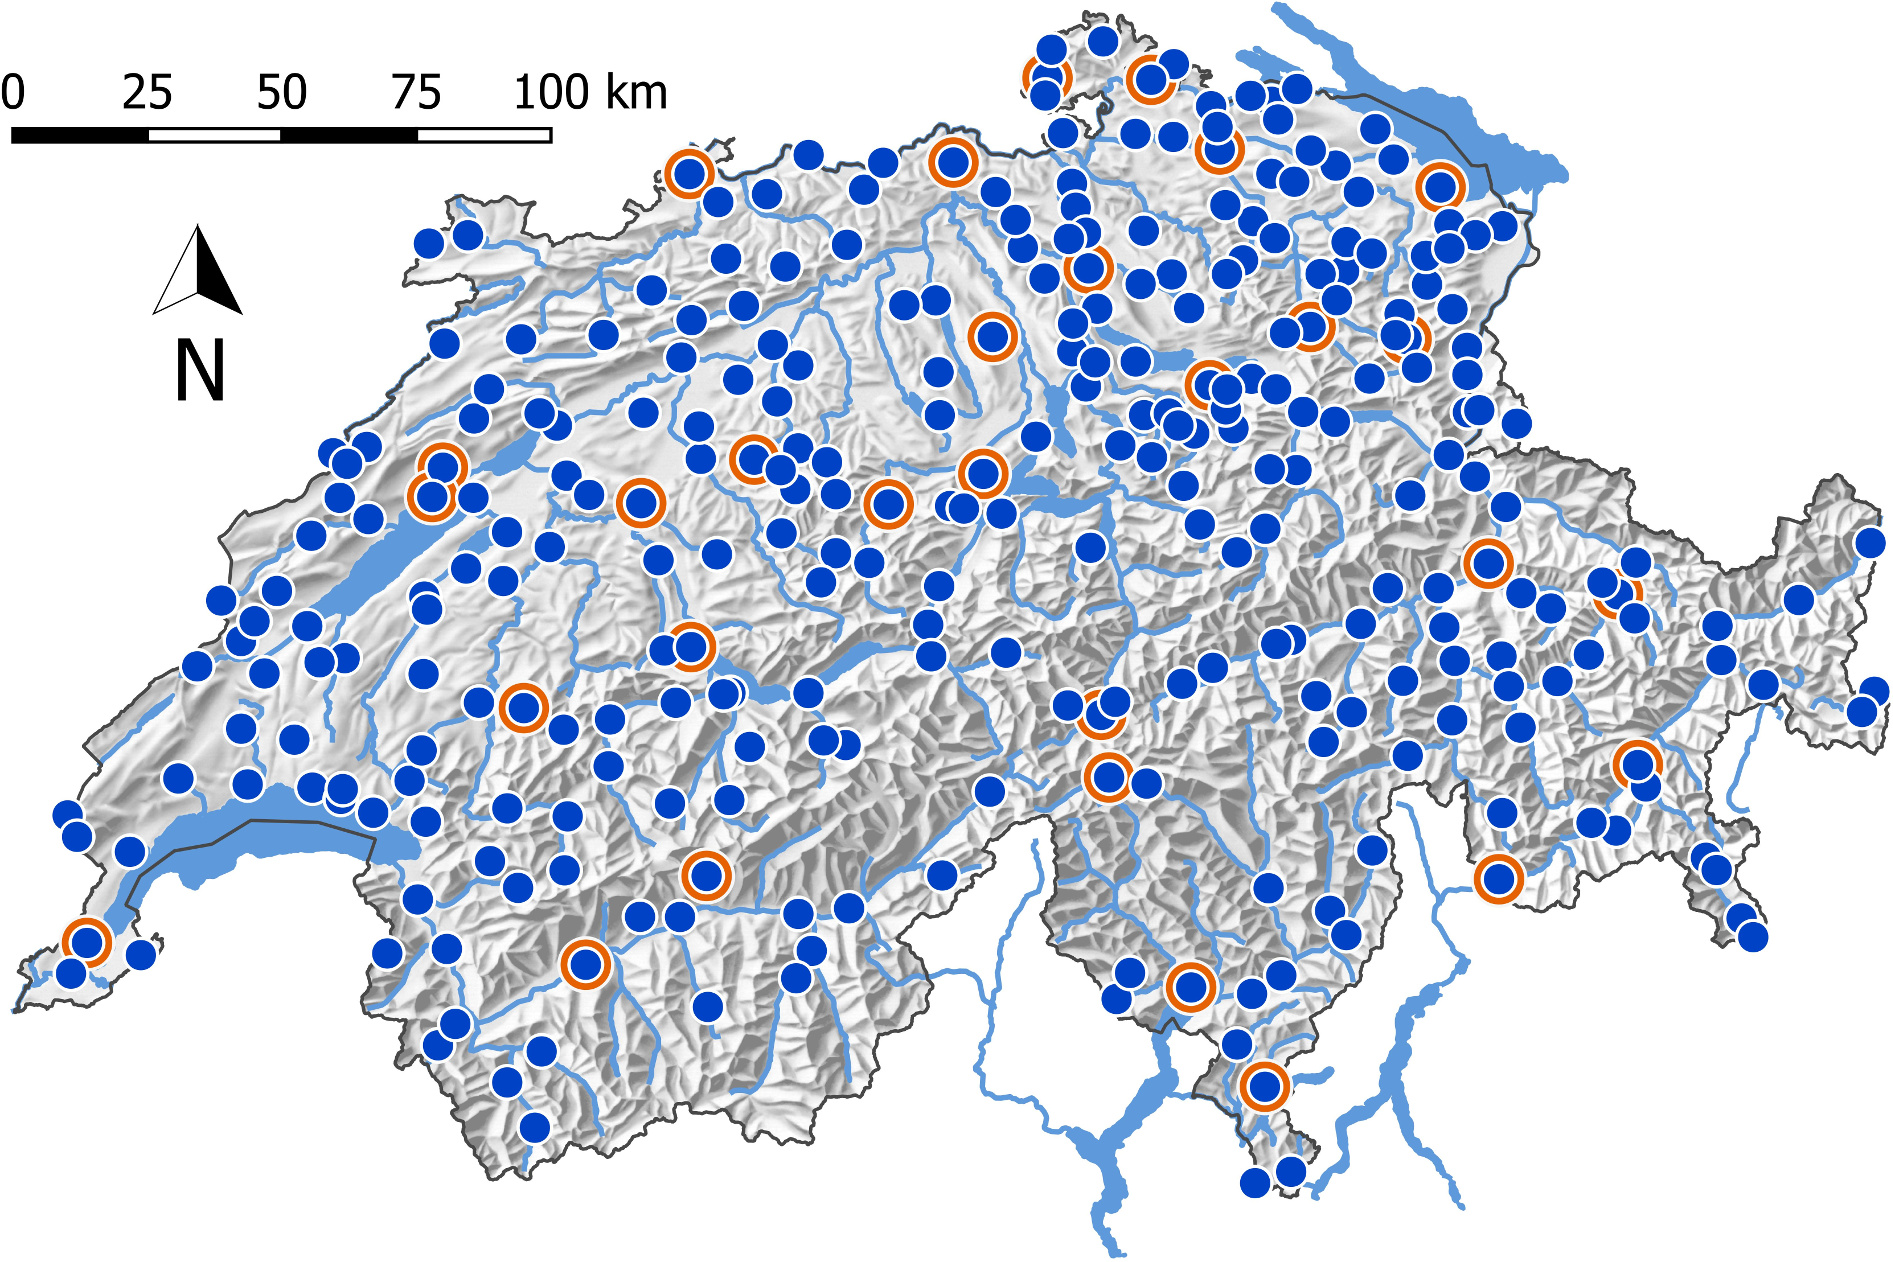
\includegraphics[width=19pc,angle=0]{figure01.pdf}\\
%\appendcaption{A1}{Caption here.}
%\end{figure}
%
% All appendix figures/tables should be placed in order AFTER the main figures/tables, i.e., tables, appendix tables, figures, appendix figures.
%
%%%%%%%%%%%%%%%%%%%%%%%%%%%%%%%%%%%%%%%%%%%%%%%%%%%%%%%%%%%%%%%%%%%%%
%  REFERENCES
%%%%%%%%%%%%%%%%%%%%%%%%%%%%%%%%%%%%%%%%%%%%%%%%%%%%%%%%%%%%%%%%%%%%%
% Make your BibTeX bibliography by using these commands:
\bibliographystyle{ametsoc2014}
\bibliography{../../../Biblio/Mendeley/Export/_For_articles-2017_JCli_reanalysis}


%%%%%%%%%%%%%%%%%%%%%%%%%%%%%%%%%%%%%%%%%%%%%%%%%%%%%%%%%%%%%%%%%%%%%
%  TABLES
%%%%%%%%%%%%%%%%%%%%%%%%%%%%%%%%%%%%%%%%%%%%%%%%%%%%%%%%%%%%%%%%%%%%%
%% Enter tables at the end of the document, before figures.
%%
%
%\begin{table}[t]
%\caption{This is a sample table caption and table layout.  Enter as many tables as
%  necessary at the end of your manuscript. Table from Lorenz (1963).}\label{t1}
%\begin{center}
%\begin{tabular}{ccccrrcrc}
%\hline\hline
%$N$ & $X$ & $Y$ & $Z$\\
%\hline
% 0000 & 0000 & 0010 & 0000 \\
% 0005 & 0004 & 0012 & 0000 \\
% 0010 & 0009 & 0020 & 0000 \\
% 0015 & 0016 & 0036 & 0002 \\
% 0020 & 0030 & 0066 & 0007 \\
% 0025 & 0054 & 0115 & 0024 \\
%\hline
%\end{tabular}
%\end{center}
%\end{table}


\begin{table*}[t]
	\caption{Considered analogue methods with increasing complexity. P0 is the preselection (PC: on calendar basis, that is $\pm 60$ days around the target date), L1, L2 and L3 are the subsequent levels of analogy. The meteorological variables are: SLP -- mean sea level pressure, Z -- geopotential height, T -- air temperature, W -- vertical velocity, MI -- moisture index, which is the product of the relative humidity at the given pressure level and the total water column. The analogy criterion is S1 for SLP and Z and RMSE for the other variables.}
	\begin{center}
		\begin{tabular}{cccccl}
			\hline
			\textbf{Method} & \textbf{P0} & \textbf{L1} & \textbf{L2} & \textbf{L3} & \textbf{Reference} \\ 
			\hline 
			\multirow{2}{*}{\textbf{2SLP}} & \multirow{2}{*}{PC} & SLP@12h &&& \\
			&& SLP@24h &&& \\
			\hline 
			\multirow{2}{*}{\textbf{2Z}} & \multirow{2}{*}{PC} & Z1000@12h &&& \multirow{2}{*}{\citealt{Bontron2004}} \\
			 && Z500@24h &&& \\
	 		\hline 
			\multirow{4}{*}{\textbf{4Z}} & \multirow{4}{*}{PC} & Z1000@06h &&& \multirow{4}{*}{\citealt{Horton2017b}} \\
			 && Z1000@30h &&& \\
			 && Z700@24h &&& \\
			 && Z500@12h &&& \\
			\hline 
			\multirow{2}{*}{\textbf{2Z-2MI}} & \multirow{2}{*}{PC} & Z1000@12h & \multirow{2}{*}{MI850@12+24h} && \multirow{2}{*}{\citealt{Bontron2004}} \\
			&& Z500@24h &&& \\
			\hline 
			\multirow{4}{*}{\textbf{4Z-2MI}} & \multirow{4}{*}{PC} & Z1000@30h &&& \multirow{4}{*}{\citealt{Horton2017b}}\\
			&& Z850@12h & MI700@24h && \\
			&& Z700@24h & MI600@12h && \\
			&& Z400@12h &&& \\
			\hline 
			\multirow{2}{*}{\textbf{PT-2Z-4MI}} & T925@36h & Z1000@12h & MI925@12+24h && \multirow{2}{*}{\citealt{BenDaoud2016}} \\
			& T600@12h & Z500@24h & MI700@12+24h && \\
			\hline 
			\multirow{2}{*}{\textbf{PT-2Z-4W-4MI}} & T925@36h & Z1000@12h & \multirow{2}{*}{W850@06-24h} & MI925@12+24h & \multirow{2}{*}{\citealt{BenDaoud2016}} \\
			& T600@12h & Z500@24h && MI700@12+24h & \\
			\hline 
			
		\end{tabular} 
	\end{center}
	\label{table:methods}
\end{table*}



\begin{table*}[t]
	\caption{Assessed reanalysis datasets with their respective properties, sorted by model age.}
	\begin{center}
		\begin{tabular}{ccccccc}
			\hline
			\multirow{2}{*}{\textbf{Name}} & \multirow{2}{*}{\textbf{Institution}} & \textbf{Period} & \textbf{Output} & \textbf{Model} & \textbf{Model} & \textbf{Assimilation}\\ 
			&& \textbf{of record} & \textbf{resolution} & \textbf{resolution} & \textbf{vintage} & \textbf{technique} \\ 
			\hline 
			\textbf{NR-1} & NCEP, NCAR & 1948 -- present & 2.5\degree x 2.5\degree & T62 ($\sim$1.88\degree), L28 & 1995 & 3D-Var\\
			\textbf{NR-2} & NCEP, DOE & 1948 -- present & 2.5\degree x 2.5\degree & T62 ($\sim$1.88\degree), L28 & 2001 & 3D-Var\\
			\textbf{ERA-INT} & ECMWF & 1979 -- present & 0.75\degree x 0.75\degree & TL255 ($\sim$0.70\degree), L60 & 2006 & 4D-Var\\
			\textbf{CFSR} & NCEP & 1979 -- present & 0.5\degree x 0.5\degree & T382 ($\sim$0.31\degree), L64 & 2009 & 3D-Var\\
			\textbf{JRA-55}  & JMA & 1958 -- present & 1.25\degree x 1.25\degree & TL319 ($\sim$0.36\degree), L60 & 2009 & 4D-Var\\
			\textbf{JRA-55C}  & JMA & 1958 -- 2015 & 1.25\degree x 1.25\degree & TL319 ($\sim$0.36\degree), L60 & 2009 & 4D-Var\\
			\textbf{20CR-2c} & NOAA-CIRES & 1851 -- 2014 & 2\degree x 2\degree & T62 ($\sim$1.88\degree), L28 & 2009 & E. K. filter\\
			\textbf{ERA-20C} & ECMWF & 1900 -- 2010 & 1\degree x 1\degree & TL159 ($\sim$1.13\degree), L91 & 2012 & 4D-Var\\
			\textbf{MERRA-2} & NASA GMAO & 1980 -- present & 0.625\degree x 0.5\degree & 0.625\degree x 0.5\degree, L72 & 2014 & 3D-Var\\
			\textbf{CERA-20C} & ECMWF & 1901 -- 2010 & 1\degree x 1\degree & T159 ($\sim$1.13\degree), L91 & 2016 & 4D-Var\\
			\hline 
		\end{tabular} 
	\end{center}
	\label{table:datasets}
\end{table*}







%%%%%%%%%%%%%%%%%%%%%%%%%%%%%%%%%%%%%%%%%%%%%%%%%%%%%%%%%%%%%%%%%%%%%
%  FIGURES
%%%%%%%%%%%%%%%%%%%%%%%%%%%%%%%%%%%%%%%%%%%%%%%%%%%%%%%%%%%%%%%%%%%%%
%% Enter figures at the end of the document, after tables.
%%
%
%\begin{figure}[t]
%  \noindent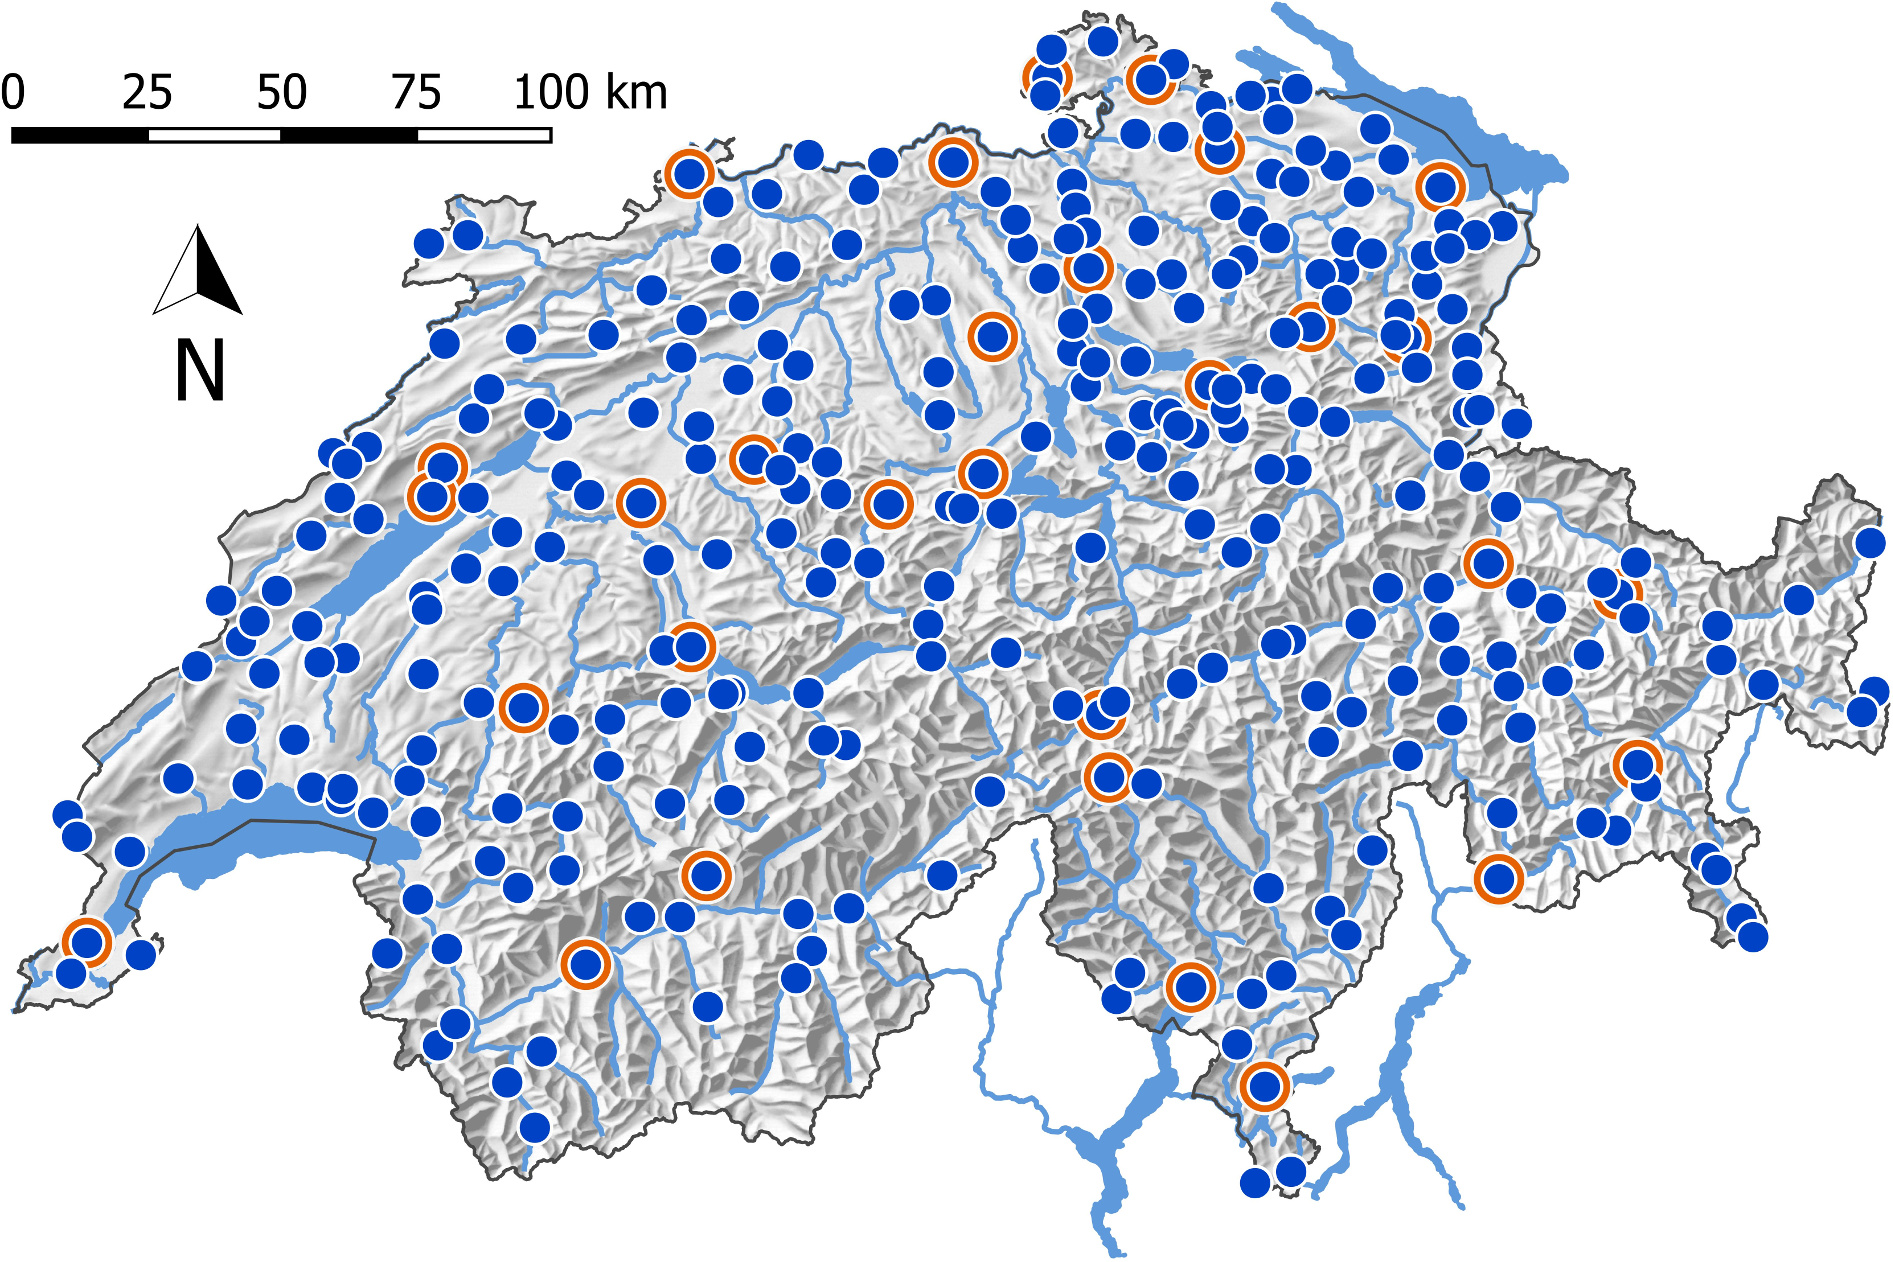
\includegraphics[width=19pc,angle=0]{figure01.pdf}\\
%  \caption{Enter the caption for your figure here.  Repeat as
%  necessary for each of your figures. Figure from \protect\cite{Knutti2008}.}\label{f1}
%\end{figure}

\begin{figure}[t]
  \noindent\includegraphics[width=19pc,angle=0]{figures/map-stations.jpg}\\
  \caption{Map of the 301 precipitation stations with a good data coverage of the period 1981--2010 (blue dots), and the 30 stations with long archives (orange). Background map: \textcopyright\ SwissTopo.}
	\label{fig:stations}
\end{figure}

\begin{figure*}[t]
	\noindent\includegraphics[width=39pc,angle=0]{figures/boxplot-per-method.pdf}\\
	\caption{CRPSS score for all stations and for all considered AMs and reanalysis datasets on the VP. A higher CRPSS score means better performance. The parameters of the AMs were calibrated for every station, every dataset, and every method. The boxes show the 25th, 50th, and 75th percentiles. The whiskers extend to the most extreme data point which is no more than 1.5 times the interquartile range.}
	\label{fig:comparison_values}
\end{figure*}

\begin{figure*}[t]
	\noindent\includegraphics[width=39pc,angle=0]{figures/boxplot-per-method-relative.pdf}\\
	\caption{Impact of the reanalysis dataset on the performance isolated by processing the improvement in CRPSS for one dataset compared to the mean performance on all datasets, per station and per method. Note that the methods cannot be compared here, only the datasets. Same conventions as Fig. \ref{fig:comparison_values}.}
	\label{fig:comparison_relative}
\end{figure*}

\begin{figure*}[t]
	\noindent\includegraphics[width=39pc,angle=0]{figures/boxplot-correl-interannual-mean.pdf}\\
	\caption{Inter-annual correlation between the mean precipitation from the selected analogues and the observations for all stations and for all considered AMs and reanalysis datasets on both the CP and the VP. Same conventions as Fig. \ref{fig:comparison_values}.}
	\label{fig:correlation}
\end{figure*}

\begin{figure*}[t]
	\noindent\includegraphics[width=39pc,angle=0]{figures/boxplot-biases-1st.pdf}\\
	\caption{Same as Fig. \ref{fig:correlation} but for the relative biases.}
	\label{fig:biases}
\end{figure*}

\begin{figure*}[t]
	\noindent\includegraphics[width=38pc,angle=0]{figures/maps-best-methods.pdf}\\
	\caption{Best method per station for the different datasets. NR-2 and JRA-55C are not shown as they are similar to NR-1 and JRA-55 respectively. Background map: \textcopyright\ SwissTopo.}
	\label{fig:map_best_methods}
\end{figure*}

\begin{figure}[t]
	\noindent\includegraphics[width=19pc,angle=0]{figures/number-analogues.pdf}\\
	\caption{Density plots of the optimal number of analogues of the last analogy level for the different AMs and datasets.}
	\label{fig:number_analogues}
\end{figure}

\begin{figure}[t]
	\noindent\includegraphics[width=19pc,angle=0]{figures/similarities-analogue-dates.pdf}\\
	\caption{Percentage of similar analogue dates selected when using the reanalysis datasets in columns that are also found when using the datasets in rows for different AMs. The values are averaged for all stations on the VP.}
	\label{fig:similarities_analogue_dates}
\end{figure}

\begin{figure}[t]
	\noindent\includegraphics[width=19pc,angle=0]{figures/plot-impact-resolution-spread.pdf}\\
	\caption{Impact (difference in CRPSS) of a decrease in grid resolution (degrees) for different datasets and AMs on the CP. The line represents the median and the shaded area represents the first and the third quartiles (on 30 stations).}
	\label{fig:plot_impact_resolution}
\end{figure}

\begin{figure}[t]
	\noindent\includegraphics[width=19pc,angle=0]{figures/plot-impact-length-spread-VP.pdf}\\
	\caption{Impact (difference in CRPSS) on the VP of an increase in the archive length (years) for different datasets and AMs. Results for the 4Z method are displayed along with the 2Z method, but with dashed lines. The line represents the median and the shaded area represents the first and the third quartiles (on 30 stations).}
	\label{fig:plot_impact_length}
\end{figure}

\begin{figure}[t]
	\noindent\includegraphics[width=19pc,angle=0]{figures/plot-impact-members-2Z.pdf}\\
	\caption{Impact (difference in CRPSS) of an increase in the number of ensemble members used for the 2Z method and for CERA-20C and 20CR-2c datasets. The results are provided for two periods: (a, c) 1981--2010 and (b, d) 1901--1930. Two approaches were assessed: (a, b) the first allowing duplicate analogue dates ("w.d.d.") and (c, d) the second without duplicate analogue dates ("wo.d.d."). The line represents the median and the shaded area represents the first and the third quartiles (on 30 stations). The dashed line and striped area correspond to results on the VP. All 56 members of 20CR-2c were assessed and the tendencies continue, but the plots are split at 30 members.}
	\label{fig:plot_impact_members_2Z}
\end{figure}

\begin{figure}[t]
	\noindent\includegraphics[width=19pc,angle=0]{figures/plot-impact-members-2Z-2MI.pdf}\\
	\caption{Same as Fig. \ref{fig:plot_impact_members_2Z} but for the 2Z-2MI method.}
	\label{fig:plot_impact_members_2Z-2MI}
\end{figure}


\end{document}